\documentclass[UTF8]{article}
\usepackage[a4paper,top=2cm,bottom=2cm,left=2.5cm,right=2cm,marginparwidth=1.75cm]{geometry}
\usepackage{xeCJK}
\usepackage{ctex}
\usepackage{fontspec}
\usepackage{float}
\usepackage{amsmath}
\usepackage{graphicx}
\usepackage[T1]{fontenc}
\usepackage{mathptmx}
\usepackage{amsmath}
\usepackage{amsfonts}
\usepackage{chemformula}
\usepackage{cite}
\usepackage[colorlinks, linkcolor=blue, anchorcolor=blue, citecolor=black]{hyperref}

\setCJKmainfont{SimSun}[AutoFakeBold,ItalicFont=KaiTi]
\title{ABABABABABA}
\author{\textup{AbaAba}}
\begin{document}
\bibliographystyle{alpha}
\begin{titlepage}
	\begin{figure}[h]
		\centering	
		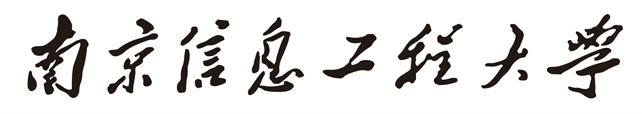
\includegraphics[width=11.32cm]{./nuist.png}
	\end{figure}
	\linespread{2.0}
	\begin{center}
		\heiti\zihao{2}寻访革命先辈足迹、探索南京历史真相
	\end{center}
	\begin{center}
		\noindent\zihao{2}《中国近现代史纲要》实践课程调查报告
	\end{center}
	~\\
	~\\
	\begin{center}\zihao{-4}
		\begin{tabular}{ll}
			\textbf{题目:}& a \\
			\textbf{年级:}& a \\
			\textbf{专业班级:}& a \\
			\textbf{组长(姓名、学号):}& a\\
			\textbf{成员(姓名、学号):}& a\\
			\textbf{完成时间:}& a\\
			\textbf{指导老师:}& a\\
		\end{tabular}
	\end{center}


	\vfill
\end{titlepage}

\part{阿巴阿巴}
\section{古诗鉴赏}
\subsection{林则徐专区}
\subsubsection{赴戍登程口占示家人}

出门一笑莫心哀,浩荡襟怀到处开。
时实难以无过立,达官非自有生来。
风涛回首空三岛,尘壤从头数九垓。
休信儿童轻薄语,嗤他赵老送灯台。

力微任重久神疲,再竭衰庸定不支。
苟利国家生死以,岂因祸福避趋之?
谪居正是君恩厚,养拙刚于戍卒宜。
戏与山妻谈故事,试吟断送老头皮。\cite{linzexu}



\bibliography{ref.bib}

\end{document}